\begin{figure*}
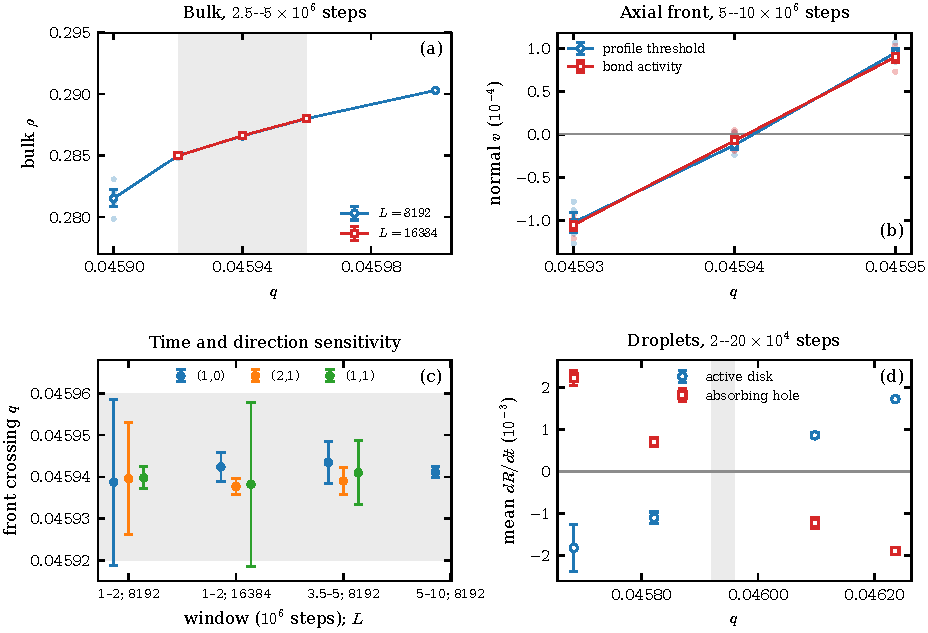
\includegraphics[width=\textwidth]{figs/fig_flagship}
\caption{Bulk and interfacial evidence at $p=\alpha=1/2$, plotted at the actual
probabilities $q$. (a) Unconditional bulk interface density, integrated over
$2.5$--$5\times10^6$ steps separately for each run, at $L=8192$ and 16384.
(b) Axial-front velocities for the independent $L=8192$, $T=10^7$ cohort,
fitted over $5$--$10\times10^6$. The profile-envelope estimate is compared
with the slope of the integrated bond activity, converted to an equivalent
width using the fixed reference density 0.2866. Four independent runs
contribute at every point in (a,b); faint symbols show individual runs and
bars give one standard error. Lines join group means.
(c) Envelope crossing estimates for the stated time windows and sizes.
The $T=2\times10^6$, $5\times10^6$, and $10^7$ cohorts are independent.
Bars are approximate pointwise delta-method Student-$t$ sensitivity intervals
with Welch--Satterthwaite degrees of freedom, conditional on the observed
bracketing pair. Small-sample coverage and bracketing uncertainty remain
limitations. All four runs must retain separated-front geometry throughout
the fit window; no invalid individual run is selectively removed.
(d) Growth rates of an active disk and an absorbing hole of initial radius
1000 on an $L=4096$ lattice, fitted over $2\times10^4$--$2\times10^5$ steps.
Bars are one standard error over four runs. The gray region in (a,c,d) is
the operational reference range $[0.04592,0.04596]$, used for normalization
sensitivity. It is not a confidence interval or an asymptotic bound.
The coarse droplet points in (d) do not resolve the smaller separations
between the front crossings in (c).}
\label{fig:flagship}
\end{figure*}
